\documentclass[conference]{IEEEtran}
\IEEEoverridecommandlockouts

% Citation management
\usepackage{cite}

% Text and list formatting
\usepackage{enumitem}
\usepackage{amsmath,amssymb,amsfonts}
\usepackage{amsthm}

% Graphics and visual elements
\usepackage{graphicx}
\usepackage{textcomp}
\usepackage{xcolor}
\usepackage{url}

% Figure and table enhancements
\usepackage{booktabs}
\usepackage{threeparttable}

% Diagrams
\usepackage{tikz}
\usetikzlibrary{arrows,positioning,fit,calc}

\newtheorem{theorem}{Theorem}
\newtheorem{lemma}{Lemma}

\newcommand{\varSpec}[3]{$#1{\times}#2{\times}#3$}

\begin{document}

\title{Solving $3\times 9$ Quoridor with Independently Verifiable Winning-Strategy Certificates}

\author{%
\IEEEauthorblockN{Ulysse Napoly}
\IEEEauthorblockA{Independent researcher \\
Correspondence: ulysse.napoly@gmail.com}
}

\maketitle

\begin{abstract}
We resolve the two previously open cells of the public Quoridor frontier table: on the $3\times 9$ board, the first player wins with 9 and with 10 walls per player, and with 10 walls the minimax forcing horizon is exactly 35 plies. The upper bound is established by a conservative audit that disables the two specialized pruning modules and proves all 18 reflection classes of the 35 second-player replies in fresh processes (9{,}309{,}248{,}724 nodes); the matching lower bound refutes every first move within 33 plies (3{,}553{,}060{,}577 nodes), and odd-ply parity excludes 34. A structurally different second solver---lazy wall-configuration construction with a union-find legality gate instead of eager enumeration---independently replicates both bounds and the 9-wall result. Beyond replication, we make the winning claim checkable without trusting any solver: a strategy-DAG certificate format (\textsf{qcert-1}) whose 18 parts (191{,}173{,}124 state--move pairs) were verified exhaustively by a clean-room verifier sharing no code with the solvers---612{,}890{,}536 verification expansions over all 35 replies, zero violations---then accepted end to end by a second independent verifier as a root-position aggregate: 287{,}795{,}827 certificate nodes, 749{,}603{,}013 regenerated edge obligations, derived bound 35, zero errors. A one-page no-stalemate theorem (height $\geq 3$, sharp at height 2) closes the one semantic loophole that could have shifted bounded verdicts. The two halves of the exact-horizon claim rest on evidence of different strength: the 35-ply upper bound is backed by independently checkable strategy certificates, while exactness additionally relies on the replicated exhaustive refutations, which are not yet certificate-backed. We also report exact partial bounds for the next open cell, $4\times 7$ with 7 walls (no forced win for either player within 26 plies), measured move-ordering effects on certified branches, and four audited negative results. All published audits are deterministic and report node counts as reproducibility fingerprints; three representative audit classes reproduced node-for-node on a second machine and compiler.
\end{abstract}

\begin{IEEEkeywords}
Quoridor, game solving, bounded adversarial search, strategy certificates, proof verification, replication
\end{IEEEkeywords}

\section{Introduction}
\label{sec:intro}

Solving a game variant exactly---determining its game-theoretic value and a witness strategy---is one of the older exact sciences of artificial intelligence, with a tradition running from Connect Four and Nine Men's Morris through checkers~\cite{allis1988knowledge,gasser1996solving,schaeffer2007checkers,herik2002games}. Quoridor has long resisted this treatment. A wall-placement race game with perfect information, it combines a large branching factor with path-legality side conditions and, on the full $9\times 9$ board, an intractable configuration space. Determining the winner of generalized $n\times n$ Quoridor was recently shown PSPACE-complete~\cite{drop2026quoridor}, by reduction from Schaefer's positive-CNF game~\cite{schaefer1978complexity}, so exact results necessarily target bounded variants.

For narrow Quoridor boards a public frontier table~\cite{slatton2026solving} records, per board geometry and wall stock, which side wins. As of this writing it lists nearly all geometries of area at most 28 as solved---with the $3\times 9$ row open at exactly two wall counts, 9 and 10 (Fig.~\ref{fig:frontier}). Those two cells are the subject of this paper.

\textbf{Results.} We show that $3\times 9$ Quoridor is a first-player win at both 9 and 10 walls per player, and that at 10 walls the win takes \emph{exactly} 35 plies against best defense (Section~\ref{sec:results}). The witness opening is the central pawn advance. Matching upper- and lower-bound audits, run with the suspect pruning modules disabled and a fresh transposition table per branch, visit 12.9 billion nodes in total; a second solver of deliberately different architecture replicates every verdict.

\textbf{The verifiability gap.} Computational game-solving results are traditionally supported by internal consistency checks and, at best, by independent re-implementation~\cite{schaeffer2007checkers,romein2003solving,henderson2009solving}. The strongest evidence practice in automated reasoning goes further: SAT solvers emit machine-checkable proof certificates that an independent---even formally verified---checker validates~\cite{wetzler2014drattrim,heule2016solving,tan2021cakelpr}, a discipline now spreading beyond SAT~\cite{elffers2020justifying}. We transport that discipline to game solving. Our solver emits a \emph{strategy-DAG certificate}: for every reachable state where the winner is to move, the move to play, with a strictly decreasing certified rank. Checking the certificate requires move generation and ply arithmetic---deterministic enumeration of the certified obligations, with no heuristic game-tree proof search---so a small clean-room program can validate the entire winning claim (Section~\ref{sec:cert}).

\textbf{Contributions.}
\begin{itemize}[leftmargin=*]
\item \textbf{C0.} First-player wins for \varSpec{3}{9}{9} and \varSpec{3}{9}{10}, closing the two open cells of the public frontier, with an exact 35-ply forcing horizon at 10 walls (certificate-backed upper bound; dual-solver replicated exhaustive lower bound).
\item \textbf{C1.} An independently checkable certificate stack (\textsf{qcert-1} parts, \textsf{qcert-aggregate-1} composition): 18 parts verified exhaustively by a clean-room verifier (zero violations over all 35 replies), and an accepted cross-architecture aggregate binding all 18 parts to the initial-position claim.
\item \textbf{C2.} A no-stalemate theorem for boards of height $\geq 3$ with a sharp height-2 counterexample, turning a documented semantics/code divergence into proved dead code for all published claims.
\item \textbf{C3.} A replication methodology---conservative audits, node-exact cross-toolchain determinism spot checks, differential validation against clean-room rule engines---reusable as an evidence standard for computational game solving.
\item \textbf{C4.} Exact partial bounds for the next open cell, \varSpec{4}{7}{7}: neither player forces a win within 26 plies; the central opening forces no first-player win within 27.
\item \textbf{C5.} Measured move-ordering effects on certified branches (2--13$\times$ node reductions), a horizon-reversal caution against shallow pilot benchmarks, and four audited negative results.
\end{itemize}

\begin{figure}[t]
\centering
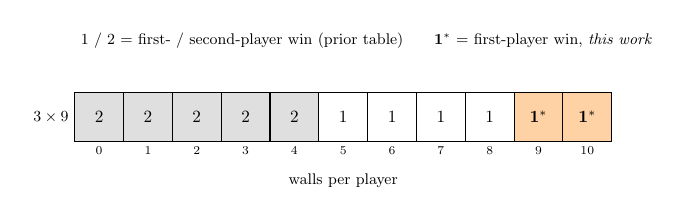
\begin{tikzpicture}[scale=0.62, every node/.style={transform shape}]
\def\cellw{1.0}
\def\newcell{N}
\foreach [count=\i from 0] \winner/\clr in {2/gray!25, 2/gray!25, 2/gray!25, 2/gray!25, 2/gray!25, 1/white, 1/white, 1/white, 1/white, N/orange!35, N/orange!35}{
  \draw[fill=\clr] (\i*\cellw, 0) rectangle ++(\cellw, 1.0);
  \ifx\winner\newcell
    \node at (\i*\cellw+0.5*\cellw, 0.5) {\textbf{1}$^{*}$};
  \else
    \node at (\i*\cellw+0.5*\cellw, 0.5) {\winner};
  \fi
  \node[below] at (\i*\cellw+0.5*\cellw, 0) {\scriptsize \i};
}
\node[left] at (0, 0.5) {\small $3\times 9$};
\node[below] at (5.5, -0.55) {\small walls per player};
\node[align=left, anchor=west] at (0, 2.05) {\small 1 / 2 = first- / second-player win (prior table)\; $\quad$ \textbf{1}$^{*}$ = first-player win, \emph{this work}};
\end{tikzpicture}
\caption{The $3\times 9$ row of the public Quoridor frontier table~\cite{slatton2026solving}. Cells 0--8 were already solved (second-player win through 4 walls, first-player win from 5); the cells at 9 and 10 walls per player were listed as unknown and are closed by this work, at 10 walls with an exact 35-ply horizon.}
\label{fig:frontier}
\end{figure}

All claims are backed by archived artifacts (commands, logs, SHA-256-pinned binaries, machine-readable audit records) in the research repositories accompanying this paper; Section~\ref{sec:limits} states precisely what remains trusted. The certificate stack covers the initial position end to end: exhaustively verified per-reply parts, plus an accepted aggregate composition binding all 18 parts to the root claim.

\section{Background and Related Work}
\label{sec:related}

\subsection{The game}

Quoridor is played on a $W\times H$ grid. Each player has a pawn; Player~1 starts at the middle of the bottom row and must reach the top row, Player~2 mirrors. A turn is either a pawn step to an adjacent unblocked cell---with straight jumps over the adjacent opponent and diagonal side-steps when the jump is blocked---or the placement of a two-segment wall from a finite personal stock. A wall may not overlap or cross existing walls and, crucially, may never cut off \emph{either} pawn from its goal row: every placement must preserve a path for both. The path-preservation rule couples wall legality to global connectivity. It is the source of most implementation risk.

We write \varSpec{W}{H}{k} for the $W\times H$ board with $k$ walls per player; moves are denoted $P(r,c)$ for pawn moves and $H(r,c)$/$V(r,c)$ for wall anchors. Throughout this paper rows are indexed $0$ to $H{-}1$ starting from Player~1's \emph{goal} side: Player~1 starts at $(H{-}1,\lfloor W/2\rfloor)$ and wins on row $0$, Player~2 mirrors. The rules convention document (\texttt{RULES.md}) fixes cell indexing, jump priority, and wall-anchor coordinates; every engine in this paper implements exactly that document, and all coordinates below use this single convention.

\subsection{Prior work on Quoridor}

Early academic work built playing agents: Glendenning tuned a linear evaluation with a genetic algorithm~\cite{glendenning2002mastering}, Mertens built a rule-based/minimax agent~\cite{mertens2006quoridor}, and Monte Carlo tree search agents followed~\cite{respall2018monte}. Exact analysis began with retrograde analysis of reduced boards, solving $5\times 5$ Quoridor with one wall each and related small variants~\cite{iwanaga2022analysis,iwanaga2023analysis}. The broadest exact effort to date is Slatton's frontier campaign~\cite{slatton2026solving}, which solved nearly all variants of area $\leq 28$ for most wall counts with a proof-number-search-related bounded solver~\cite{allis1994proof} over precomputed wall-configuration masks. It published the frontier table this paper extends, and it reports a structural finding we can confirm from the outside: on odd-height boards the winner flips from the second to the first player as wall stocks grow (Fig.~\ref{fig:frontier}). Our two new cells continue the first-player regime. The 10-wall horizon of exactly 35 plies quantifies the margin.

\subsection{Evidence standards in game solving}

Landmark solved-game results---Connect Four~\cite{allis1988knowledge}, Nine Men's Morris~\cite{gasser1996solving}, Kalah~\cite{irving2000solving}, Awari~\cite{romein2003solving}, small Go boards~\cite{vanderwerf2003solving}, checkers~\cite{schaeffer2007checkers}, $8\times 8$ Hex~\cite{henderson2009solving} (the general game being PSPACE-complete~\cite{even1976combinatorial,reisch1981hex}), Gardner minichess~\cite{mhalla2013gardner}---rest on careful internal validation and occasionally independent re-implementation, but none ships an artifact that a third party can check \emph{without} re-running search. The SAT community closed the analogous gap with proof logging: DRAT certificates checked by independent tools~\cite{wetzler2014drattrim}, scaled to the 200-terabyte Pythagorean-triples proof~\cite{heule2016solving}, hardened by formally verified checkers~\cite{tan2021cakelpr}, and extended beyond SAT via pseudo-Boolean justifications~\cite{elffers2020justifying}.

Two neighboring communities, moreover, have long produced what are formally strategy certificates. A quantified Boolean formula \emph{is} a two-player game between an existential and a universal player~\cite{schaefer1978complexity}, and QBF solvers routinely extract winning strategies as Skolem or Herbrand functions---circuits validated by an external SAT call, independently of the solver that produced them~\cite{balabanov2012unified,niemetz2012resolution}, with QRAT proof logging covering even aggressive preprocessing~\cite{heule2014efficient}. In constraint programming and combinatorial optimisation, pseudo-Boolean proof logging now certifies symmetry and dominance pruning~\cite{bogaerts2023certified}---the abstract counterparts of the mirror transport and wall-stock dominance table used here.

For board games the natural certificate is the same object---a winning strategy annotated so that its correctness is locally checkable---and Section~\ref{sec:cert} instantiates it for bounded Quoridor proofs. To our knowledge, no prior result in \emph{classical board-game} solving at this scale, a lineage whose landmarks rest on internally validated search, has been delivered with a solver-independent, exhaustively checked strategy certificate. The contribution is thus a bridge rather than an invention: it imports the proof-logging standards of SAT, QBF, and certified optimisation into a domain whose global path-preservation legality resists direct encoding into clauses or pseudo-Boolean constraints without combinatorial blow-up, so the certificate must speak the game's native language of moves and connectivity.

\section{Rules Semantics and the Stalemate Theorem}
\label{sec:semantics}

\subsection{Bounded proof semantics}

All solvers in this paper decide the bounded predicate $\mathrm{Win}(s,T,d)$: from state $s$, can player $T$ force a win within $d$ plies? The recursion is existential at $T$'s turns and universal at the opponent's, with terminal wins checked at entry and depth measured in plies. Transposition entries store monotone facts (``$T$ wins within $d_1$'', ``$T$ does not win within $d_2$'')~\cite{zobrist1970new,knuth1975analysis}; keeping the remaining depth in the state avoids the graph-history-interaction pathology~\cite{kishimoto2004general}. Because a first-player win can end only on an odd ply, exact horizons follow from an upper bound at $d$ and an exhaustive refutation at $d-2$.

One documented divergence existed between the semantics document and the implementations: the value of a universal node with \emph{zero legal moves} (a stalemate). The mathematical convention (empty conjunction) makes it a win for $T$; the code returns \texttt{false} for both targets. If stalemates were reachable, bounded verdicts could depend on the convention. We close this loophole with a theorem rather than an assumption.

\subsection{The no-stalemate theorem}

Call a state \emph{legal} if the pawns occupy distinct cells and each pawn's cell is wall-connected to some cell of its own goal row---the exact enumeration domain of the exhaustive audits, a strict superset of the reachable states (on \varSpec{4}{3}{3}: 63{,}184 legal non-terminal states versus 62{,}732 reachable).

\begin{lemma}[path invariant]
In every reachable state, each pawn is wall-connected to its goal row (walls block edges; pawns do not).
\end{lemma}

\begin{theorem}[no stalemate, $H\geq 3$]
\label{thm:stalemate}
On any board with $H\geq 3$, any width and any wall stocks, every legal non-terminal state grants the player to move at least one pawn move.
\end{theorem}

\begin{proof}[Proof sketch]
Suppose the mover $A$ at cell $p$ has no pawn move. Since the state is non-terminal and legal, $p$'s component contains a goal-row cell other than $p$, so $p$ has an unblocked neighbor; if that neighbor were empty it would be a legal step, so $p$'s \emph{only} unblocked neighbor is the opponent's cell $n$. The failed jump and both failed diagonals then force every edge at $n$ other than $n$--$p$ to be blocked or out of bounds, so the component of $p$ is exactly $\{p,n\}$. Applying legality \emph{twice}---once per pawn---this two-cell prison must contain a cell of row $0$ and a cell of row $H-1$; adjacency gives $H\leq 2$. \qedhere
\end{proof}

Two features of the proof matter. First, it needs \emph{both} pawns' connectivity: the mover-only argument (``the first vertex of the mover's shortest path is free, jumpable, or bypassable'') is irreparable, because the mover's path may legitimately run through the opponent's cell. Second, it never uses the geometric wall-placement rules, only connectivity, so it covers the audits' enumeration domain a fortiori. The full one-page proof, including the jump/diagonal edge case analysis, is archived with the artifacts.

\begin{figure}[t]
\centering
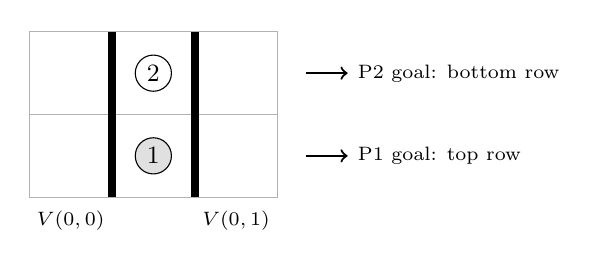
\begin{tikzpicture}[scale=1.05]
% board 3 wide (cols 0..2), 2 tall (rows 0 top,1 bottom)
\foreach \c in {0,1,2}{
  \foreach \r in {0,1}{
    \draw[gray!60] (\c, -\r) rectangle ++(1,-1);
  }
}
% pawns: P2 at (0,1) top middle; P1 at (1,1) bottom middle
\node[circle, draw, fill=white, inner sep=2pt] at (1.5, -0.5) {\small 2};
\node[circle, draw, fill=black!12, inner sep=2pt] at (1.5, -1.5) {\small 1};
% wall V(0,0): between col0 and col1, spanning both rows
\draw[line width=3pt] (1, 0) -- (1, -2);
% wall V(0,1): between col1 and col2, spanning both rows
\draw[line width=3pt] (2, 0) -- (2, -2);
\node[below] at (0.5, -2.05) {\scriptsize $V(0,0)$};
\node[below] at (2.5, -2.05) {\scriptsize $V(0,1)$};
\draw[->, thick] (3.35, -0.5) -- (3.85, -0.5) node[right] {\scriptsize P2 goal: bottom row};
\draw[->, thick] (3.35, -1.5) -- (3.85, -1.5) node[right] {\scriptsize P1 goal: top row};
\end{tikzpicture}
\caption{Sharpness at $H=2$: on the $3\times 2$ board, $V(0,0)$ then $V(0,1)$ (thick segments) seal the central column. Player~1 (to move) has no pawn move---the only unblocked neighbor is occupied, the jump lands out of bounds, both diagonals are blocked---and both wall anchors are used, so no move exists at all, even with walls in stock. Both pawns still satisfy the legality invariant, sitting on each other's goal rows: exactly the two-cell prison the theorem's final step excludes for $H\geq 3$.}
\label{fig:stalemate}
\end{figure}

\subsection{Sharpness, mechanical verification, consequences}

The bound is sharp: Fig.~\ref{fig:stalemate} shows a stalemate reachable in two plies on the $3\times 2$ board. On height-2 boards the convention is semantically live---exhaustive dual-convention solves measure 7, 12, and 42 diverging state verdicts on \varSpec{3}{2}{1}, \varSpec{3}{2}{2}, and \varSpec{4}{2}{2} respectively---so height-2 claims must fix the convention explicitly. For $H\geq 3$ the divergent branch is dead code.

The theorem was verified mechanically by a clean-room engine (Table~\ref{tab:scans}): forward scans of all reachable states, direct enumerations of the legal superset (independently reproducing the archived 63{,}184 count on \varSpec{4}{3}{3}), and an adversarial hunt over degenerate topologies with a pawn-move generator re-implemented from the rules document alone. Every $H\geq 3$ scan found zero pawn-move-less states; $H=2$ controls found stalemates exactly as constructed. Every production audit additionally archives a \texttt{stalemates\_seen} counter, pinned to zero as a runtime tripwire.

\begin{table}[t]
\centering
\caption{Mechanical verification of Theorem~\ref{thm:stalemate} (clean-room engine, archived scans).}
\label{tab:scans}
\begin{tabular}{lrr}
\toprule
Scan family & States & Pawn-move-less \\
\midrule
Reachable, 15 variants, $H\geq 3$ & $\approx$1.9M & 0 \\
Legal superset, 8 variants, $H\geq 3$ & $\approx$3.4M & 0 \\
Adversarial hunt, 9 topologies & $\approx$17.8M & 0 \\
$H=2$ negative controls & --- & found at ply 2 \\
\bottomrule
\end{tabular}
\end{table}

\section{Solvers and Audit Methodology}
\label{sec:method}

Two exact solvers of deliberately different architecture, three clean-room rule implementations, and a layered audit protocol produce and check every claim (Fig.~\ref{fig:stack}).

\begin{figure}[t]
\centering
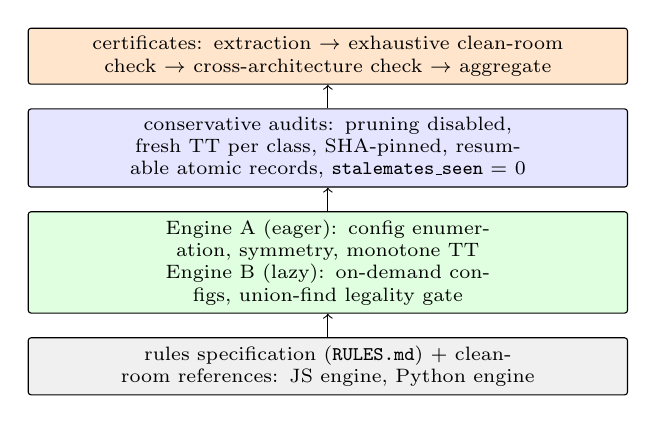
\begin{tikzpicture}[
  box/.style={draw, rounded corners=1pt, align=center, font=\scriptsize, inner sep=3pt, text width=74mm},
  node distance=3mm
]
\node[box, fill=orange!20] (cert) {certificates: extraction $\to$ exhaustive clean-room check $\to$ cross-architecture check $\to$ aggregate};
\node[box, fill=blue!10, below=of cert] (audit) {conservative audits: pruning disabled, fresh TT per class, SHA-pinned, resumable atomic records, \texttt{stalemates\_seen} = 0};
\node[box, fill=green!12, below=of audit] (engines) {Engine A (eager): config enumeration, symmetry, monotone TT \\ Engine B (lazy): on-demand configs, union-find legality gate};
\node[box, fill=gray!12, below=of engines] (rules) {rules specification (\texttt{RULES.md}) + clean-room references: JS engine, Python engine};
\draw[->] (rules) -- (engines);
\draw[->] (engines) -- (audit);
\draw[->] (audit) -- (cert);
\end{tikzpicture}
\caption{The evidence stack. Differential grids tie every layer back to the rules specification; the certificate layer at the top is checkable without trusting anything below it except the rules reading and ply arithmetic.}
\label{fig:stack}
\end{figure}

\subsection{Engine A: eager enumeration}

The primary solver pre-enumerates all legal wall configurations of the variant (2{,}929{,}319 for \varSpec{3}{9}{10}; 16{,}368{,}423 for \varSpec{4}{7}{7}) and stores, per configuration, goal reachability, distances, movement edges, legal wall additions, and symmetry transforms. Search is the bounded existential/universal recursion---AND/OR proof search in the tradition of~\cite{allis1994proof,allis1994searching}---with iterative deepening, horizontal-mirror and 180$^\circ$ player-swap symmetry, depth-parity normalization, and a two-slot transposition table with full-key equality. Move ordering affects performance only; verdicts are ordering-invariant, a property the portfolio harness enforces by construction (Section~\ref{sec:ordering}).

\subsection{Engine B: lazy replication solver}

The replication solver was written against the rules and semantics documents with a deliberately different design. It never enumerates the configuration universe, building wall configurations only when the current proof obligation reaches them. Wall legality is decided by an $O(\alpha)$ union-find cycle gate over the junction lattice: a wall can disconnect a pawn only by closing a cycle with existing walls or the border, each wall contributes two half-segments, and a placement is safe when no cycle closes; BFS runs only in the rare cycle-closing cases. A built-in self-test compares the gate against BFS on 121{,}418 legality verdicts with zero divergence. Profiling confirms the design premise: a single proof branch touches 0.3--4.6\% of the configuration universe.

\subsection{Audit protocol}

Every published bound comes from a \emph{conservative audit}, extending the internal-validation practice of earlier solved-game efforts~\cite{schaeffer2007checkers,romein2003solving}: the two specialized pruning modules most deserving suspicion---the admissible distance bound and the pawn-only endgame table---are disabled; each decomposed class runs in a fresh process with a fresh transposition table; binaries are SHA-256-pinned; every record is written atomically and the harness resumes idempotently; and each record archives node counts, depths, timings, and the theorem-backed \texttt{stalemates\_seen}=0 counter. Class manifests are re-parsed from the binary and hash-bound, so an ordering change cannot silently move a historical representative.

\subsection{Differential validation}

Table~\ref{tab:validation} summarizes the validation grids. The two reference engines were independently implemented from the frozen rules and proof-semantics specifications, without consulting or reusing production-solver source code: the JS engine was written from \texttt{RULES.md} and \texttt{PROOF\_SEMANTICS.md} alone, without reading the C++ or Python sources, and independently re-derives the wall-configuration counts by transfer-matrix dynamic programming. Six fully solved small variants match the public table~\cite{slatton2026solving}, a fourth independent source for those values.

\begin{table}[t]
\centering
\caption{Differential validation inventory (all archived; zero divergence throughout).}
\label{tab:validation}
\begin{tabular}{lr}
\toprule
Check & Scale \\
\midrule
Exhaustive legal-move grid, \varSpec{4}{3}{3} & 63{,}184 states \\
Random move grids, \varSpec{3}{9}{10} / \varSpec{4}{7}{7} & 2{,}000 / 1{,}500 states \\
Exhaustive bounded-proof grid, \varSpec{3}{3}{1} & 51{,}408 queries \\
Sampled proof grid, \varSpec{4}{3}{2} & 5{,}000 queries \\
Known-variant regressions (both winners) & 6 variants \\
Wall universes, independent recount & 2 variants \\
Root/reply reflection partitions & re-derived \\
Sanitizers (ASan, UBSan), Clang rebuilds & tractable suites \\
Union-find gate vs.\ BFS (Engine B) & 121{,}418 verdicts \\
\bottomrule
\end{tabular}
\end{table}

\subsection{Determinism as a reproducibility fingerprint}

The search is deterministic and portable: re-running archived audit commands on a different machine, compiler, and freshly compiled binary reproduces node counts \emph{exactly} (three classes checked: 79{,}766{,}979, 142{,}908{,}257, and 44{,}048{,}383 nodes). We report node counts throughout as fingerprints that any replicator can match bit-for-bit; the claims themselves rest on verdicts, not counts.

\section{Results: The $3\times 9$ Frontier Cells}
\label{sec:results}

\begin{table*}[t]
\centering
\caption{The \varSpec{3}{9}{10} bounds and their independent replication. Upper audits prove all 18 reflection classes of the 35 replies to the witness opening; lower audits refute all 18 first-move classes within 33 plies. Engine A audits disable the distance bound and pawn-only table with a fresh TT per class.}
\label{tab:bounds}
\begin{threeparttable}
\begin{tabular}{llrrr}
\toprule
Bound & Solver & Classes & Nodes & Search time (s) \\
\midrule
Upper: win $\leq 35$ & Engine A (conservative audit) & 18/18 & 9{,}309{,}248{,}724 & 1{,}805.6 \\
Upper: win $\leq 35$ & Engine B (per-class TT) & 18/18 & 5{,}402{,}042{,}173 & --- \\
Lower: no win $\leq 33$ & Engine A (conservative audit) & 18/18 & 3{,}553{,}060{,}577 & 716.5 \\
Lower: no win $\leq 33$ & Engine B & 18/18 & 2{,}505{,}091{,}973 & 1{,}171 \\
\midrule
\varSpec{3}{9}{9} upper: win $\leq 35$ & Engine A (monolithic + 18-class) & 18/18 & 1{,}909{,}467{,}037\tnote{a} & 452.3 \\
\varSpec{3}{9}{9} upper: win $\leq 35$ & Engine B & 18/18 & 6{,}577{,}365{,}458 & --- \\
\bottomrule
\end{tabular}
\begin{tablenotes}\footnotesize
\item[a] Monolithic run; the decomposed 18-class verification is archived separately (slowest class 2{,}514{,}031{,}626 nodes).
\end{tablenotes}
\end{threeparttable}
\end{table*}

\subsection{$3\times 9$, 10 walls: a first-player win in exactly 35 plies}

After the central opening $P(7,1)$ (the pawn advance $(8,1)\!\to\!(7,1)$), Player~2 has 35 legal replies, which horizontal reflection partitions into 18 exact classes; the partition is re-derived by independent scripts. The conservative audit proves every representative in a fresh process. That gives the 35-ply upper bound from the initial position. The lower-bound audit fixes each of the 18 reflection classes of Player~1's first moves and exhaustively refutes a win within the remaining 32 plies---no proof, no timeout---so no first-player win exists within 33 plies. Wins for Player~1 occur only on odd plies, excluding 34. Hence the minimax forcing horizon is exactly 35. The two halves of this statement carry evidence of different strength: the upper bound is additionally certificate-backed (Section~\ref{sec:cert}), while the 33-ply refutations rest on the dual-solver exhaustive audits. Table~\ref{tab:bounds} gives the numbers for both engines. The two architectures agree on all 36 verdicts and on the fine structure of the proof: 17 classes prove at remaining depth 31 and the retreat reply $P(1,1)$ alone requires 33, in both engines and at both wall counts.

\subsection{$3\times 9$, 9 walls}

The same protocol proves the first-player win at 9 walls (upper bound 35), covering the second open cell. The public table records winners, not horizons~\cite{slatton2026solving}; our lower-bound replication at 10 walls completes the exact-horizon statement where it is claimed.

\subsection{What replication adds}

Engine B shares no search code, no state representation, no configuration enumeration, and no wall-legality algorithm with Engine A. Its agreement on all 54 decomposed class verdicts across the two variants---36 upper-bound classes and 18 lower-bound refutations---makes a correlated \emph{search} defect implausible; the remaining single point of failure---a shared misreading of the rules---is addressed by the clean-room differential grids of Table~\ref{tab:validation} and, more strongly, by the certificates of the next section.

\section{Independently Verifiable Certificates}
\label{sec:cert}

Replication still asks a skeptic to trust two searches. The certificate layer removes that trust: it packages the winning strategy itself in a form checkable by deterministic exhaustive enumeration of the certified obligations---no heuristic game-tree proof search, no solver code (Fig.~\ref{fig:certpipe}).

\subsection{Format}

A \textsf{qcert-1} certificate is a JSONL strategy DAG for a claim ``player $T$ wins from root $r$ within $d$ plies.'' Each line is one deduplicated state with its certified rank; at states where $T$ moves it declares the strategy move. The verifier's obligations are purely local: the root is present at rank $\leq d$; at every $T$-node the declared move is legal and leads to a node of strictly smaller rank (or an immediate terminal win); at every opponent node \emph{all} legal replies are covered by nodes of strictly smaller rank; terminal states are wins for $T$. Rank strict decrease makes well-foundedness a syntactic property---no cycle can certify---and the ply bound becomes arithmetic on ranks. The format stores certified ranks rather than exact distances-to-mate: any consistent decreasing assignment is sound, which keeps emission cheap. A hardened lexical layer (UTF-8 without BOM, safe-integer grammar, gzip integrity binding) is shared by all verifiers; adversarial corpora of 10, 20, and 33 corruption families are rejected by the in-memory, streaming, and aggregate verifiers respectively. The local-obligation design deliberately mirrors clausal proof checking in SAT~\cite{wetzler2014drattrim}, whose certificates have scaled to hundreds of terabytes~\cite{heule2016solving}.

\begin{figure}[t]
\centering
\resizebox{\columnwidth}{!}{%
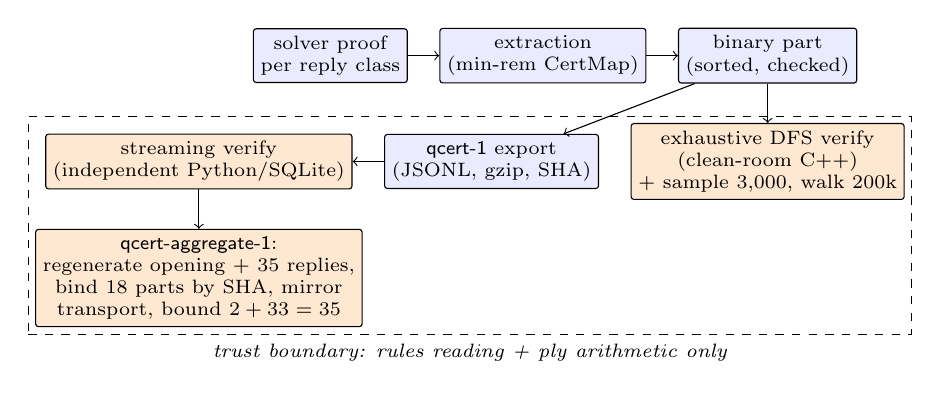
\begin{tikzpicture}[
  stage/.style={draw, rounded corners=1pt, align=center, font=\scriptsize, inner sep=2.6pt, fill=blue!8},
  vstage/.style={draw, rounded corners=1pt, align=center, font=\scriptsize, inner sep=2.6pt, fill=orange!18},
  node distance=2.6mm and 4mm
]
\node[stage] (memo) {solver proof\\per reply class};
\node[stage, right=of memo] (cert2) {extraction\\(min-rem CertMap)};
\node[stage, right=of cert2] (part) {binary part\\(sorted, checked)};
\node[vstage, below=5mm of part] (qverify) {exhaustive DFS verify\\(clean-room C++)\\+ sample 3{,}000, walk 200k};
\node[stage, left=of qverify] (export) {\textsf{qcert-1} export\\(JSONL, gzip, SHA)};
\node[vstage, left=of export] (sqlite) {streaming verify\\(independent Python/SQLite)};
\node[vstage, below=5mm of sqlite] (agg) {\textsf{qcert-aggregate-1}:\\regenerate opening + 35 replies,\\bind 18 parts by SHA, mirror\\transport, bound $2+33=35$};
\draw[->] (memo) -- (cert2);
\draw[->] (cert2) -- (part);
\draw[->] (part) -- (qverify);
\draw[->] (part) -- (export);
\draw[->] (export) -- (sqlite);
\draw[->] (sqlite) -- (agg);
\node[draw, dashed, inner sep=2.5pt, fit=(qverify)(sqlite)(agg), label={[font=\scriptsize\itshape]below:trust boundary: rules reading + ply arithmetic only}] {};
\end{tikzpicture}%
}
\caption{Certificate pipeline. Emission (blue) may use solver data structures; every verifier (orange) is independent of the solvers---the exhaustive C++ verifier shares zero code with them, and the streaming verifier was written by the other research line against the format specification.}
\label{fig:certpipe}
\end{figure}

\subsection{Extraction and the min-rem invariant}

Parts are extracted per reply class from the prover's memo. One extraction bug became a design rule. When the same state is certified twice---once deep inside a proof with a tight remaining budget, once shallowly with a loose one---keeping the \emph{larger} budget's entry can create rank plateaus that let the merged strategy cycle between certified states (observed as a two-state loop between $P(3,2)$ and $P(4,2)$). The fix is a single invariant: the certificate map only ever keeps the \emph{minimum} remaining-ply certification per state. This min-rem rule restores strict decrease by construction, and a forensic reproducer for the pre-fix behavior is archived. For the same reason we do \emph{not} claim the merged single-file strategy: min-per-key merging across parts mixes tempi, with rare rank violations measured at roughly one per 900 states. The deliverable is the 18 per-class parts, which are individually self-contained.

\subsection{Verification results}

Table~\ref{tab:cert} summarizes. The 18 parts cover all 35 legal replies: 18 canonical representatives verified directly and 17 mirror twins verified by applying the reflection automorphism from ply 1 (an earlier intra-part mirror fallback was found unsound and removed). The exhaustive pass uses a clean-room C++ verifier---a port of the Python reference checker sharing zero code with either solver---and performs 612{,}890{,}536 verification expansions across the 35 branches with zero violations, in 1{,}262.6~s. Mirror-twin pairs exhibit identical memo cardinalities, an isomorphism consistency check that comes for free.

Cross-architecture validation bridges the two research lines. The $H(1,0)$ part was exported to \textsf{qcert-1} (881{,}735{,}925 bytes, SHA-256-pinned; the export is bit-reproducible from the memo) and accepted by the \emph{other} line's independently written streaming verifier: 9{,}836{,}857 nodes, 25{,}175{,}363 regenerated edges, root budget 31, zero errors, 1{,}239~s. That verifier regenerates every move obligation from the independent Python rules engine against a disk-backed index. A further differential drew 1{,}500 wall configurations from the accepted index and compared the optimized connectivity profiles against naive BFS: 10{,}024 legal moves and 706{,}806 all-cell goal-connectivity checks, zero divergence.

\begin{table}[t]
\centering
\caption{Certificate verification for \varSpec{3}{9}{10} (witness opening $P(7,1)$; 18 parts, 191{,}173{,}124 state--move pairs).}
\label{tab:cert}
\setlength{\tabcolsep}{3pt}
\begin{tabular}{lrr}
\toprule
Check & Scale & Viol. \\
\midrule
Sampled adversary games (per part) & $18\times 3{,}000$ & 0 \\
Bounded DFS walks (per part) & $18\times 200{,}000$ & 0 \\
Exhaustive clean-room pass & 35/35; 612.9M expansions & 0 \\
Cross-arch.\ acceptance of $H(1,0)$ & 9.84M nodes, 25.2M edges & 0 \\
Profile differential on $H(1,0)$ & 706{,}806 checks & 0 \\
18-part aggregate acceptance & 287.8M nodes, 749.6M edges & 0 \\
\bottomrule
\end{tabular}
\end{table}

\subsection{Composing parts into the root claim}

Eighteen branch certificates do not yet formally certify the initial position; the missing step is bookkeeping, and it too is specified and independently checkable. A \textsf{qcert-aggregate-1} manifest regenerates the witness opening and the exact set of 35 replies, binds each reply orbit to its part by stored-byte SHA-256, transports mirror-twin strategies through the documented reflection automorphism (one reply is self-mirror), verifies each part with a fresh index, and derives the bound $2 + 33 = 35$ explicitly. The aggregate verifier rejects 33 corruption families, including path aliasing and manifest tampering, and is validated end to end on a small complete fixture.

The production aggregate over the 18 real parts has been accepted. Every part passed under both the identity and mirror-columns transforms---287{,}795{,}827 certificate nodes in total, exactly matching the extraction-memo state count, with 749{,}603{,}013 regenerated edge obligations---the 35 replies were regenerated and matched to their 18 orbits, and the bound was derived explicitly as $2+33=35$, in 30{,}232~s under the SHA-frozen streaming verifier (Table~\ref{tab:cert}, last row). The initial-position claim is therefore certificate-backed end to end. One bookkeeping note: the aggregate's $H(0,0)$ part is a regenerated, equally verified strategy, distinct from the archived binary part used in the exhaustive pass; the two are valid alternatives whose cardinalities must not be summed.

\subsection{Trust boundary}

What must a skeptic still trust? (i) that \texttt{RULES.md} captures the intended game---checked socially, and against the public table on six solved variants; (ii) the verifier they choose to run---each is small, search-free, and available in three independent implementations (in-memory JS, streaming Python/SQLite, exhaustive C++), written by different parties, two of them clean-room; and (iii) ply arithmetic. Notably \emph{excluded} from the trusted base: both solvers, the transposition logic, the symmetry code, the pruning modules, and the extraction pipeline. The lower bound (no win within 33) is the one claim not yet certificate-backed; it rests on the dual-solver exhaustive refutations, and Section~\ref{sec:limits} sketches survival certificates as the designed remedy.

\section{Frontier Progress on $4\times 7$ Quoridor}
\label{sec:fourseven}

The next open cell in the same table~\cite{slatton2026solving} is $4\times 7$ with 7 walls per player. It remains open, but exact partial bounds now constrain it (Table~\ref{tab:fourseven}): fixing each of Player~1's 39 legal first moves and refuting a win in the remaining 24 plies shows no first-player win within 25 plies; a completed Player-2 audit through depth 26 shows no second-player win within 26; and after the central exchange $P(5,2)$, $P(1,2)$, all 40 third moves are refuted at the remaining 24-ply bound, so the central opening forces no win within 27 plies. All audits use the conservative protocol (pruning disabled, fresh 64-bit-keyed tables). A memory redesign (deriving the opponent's distance tables by exact 180$^\circ$ rotation instead of storing both) cut precompute RSS from 2.95 to 2.15~GiB and, reproducing archived branches node-exactly, enables larger transposition tables for the coming campaigns.

\begin{table}[t]
\centering
\caption{Exact partial bounds for \varSpec{4}{7}{7} (game value open).}
\label{tab:fourseven}
\begin{tabular}{lrr}
\toprule
Audit & Branches & Nodes \\
\midrule
P1 root refutation $\leq 25$ plies & 39/39 & 4{,}888{,}712{,}130 \\
P2 refutation $\leq 26$ plies & complete & 901{,}837{,}164 \\
Central opening refuted $\leq 27$ & 40/40 & 3{,}591{,}324{,}070 \\
\bottomrule
\end{tabular}
\end{table}

\section{Ordering Portfolios and Negative Results}
\label{sec:ordering}

With certified branches available, move-ordering policies can be raced under a hard soundness constraint: same named branch, same verdict, fresh tables. Two findings and four audited negatives came out of this harness (Table~\ref{tab:ordering}).

\textbf{Path-flow ordering.} Scoring candidate walls by their impact on the opponent's whole shortest-path DAG (how many shortest routes an edge carries) is a strong exact ordering signal in corridor positions: on the archived $P(4,2)$ branch of \varSpec{4}{7}{7} it cuts the proof from 119.9M to 47.2M nodes, and on two certified \varSpec{3}{9}{10} replies it roughly halves nodes and wall time. In the lazy engine, a related route-choice count ordering cuts a hard branch from 223.2M nodes (47.3~s) to 15.3M (3.7~s), and combining it with an exact wall-stock dominance table (a Pareto argument: extra own walls never hurt, extra opponent walls never help) reaches 12.9M nodes.

\textbf{Horizon reversal.} The same harness produced a caution: on $P(4,2)$, the policy that wins at shallow pilot depths \emph{loses} at full depth. Policy selection from shallow pilots is unsound in this domain; portfolios must race at the target horizon with stable named moves (an earlier negative diagnosis of this very signal was itself invalidated because index-based move naming let the ordering change the tested position).

\textbf{Exact race endgames.} Once wall stocks are exhausted, Quoridor reduces to a pure pawn race, and this subgame turns out to admit a complete, exactly verified characterization. Sweeping the full fixed-point race tables of 24 boards ($W\in\{2,3,5,9\}$, $H\in\{4,\dots,9\}$; the $9\times 9$ table self-checks against an independently validated implementation on all 10{,}242 states) establishes a dichotomy: with equal goal distances $d$, the player to move \emph{loses}---in exactly $2d$ plies---if and only if the pawns face each other on the same column with an even row gap (possible only on odd-height boards, where the initial position is the extreme case), and \emph{wins} in every other equal-distance configuration; no drawn race state exists on any swept board. The mechanism is tempo: a blocked face-to-face jump hands over exactly one tempo, so column alignment at even gap is pure zugzwang. The dichotomy is established computationally and backed by a complete imitation-strategy proof in the artifacts (a jump-tempo lemma, a contact-parity invariant, and an interception lemma); the proof was then attacked by an independent adversarial audit, which pierced three minor gaps---including a genuine accounting error omitting backward jumps---that were repaired with the audit trail preserved in the same document. Practically, the characterization is a three-comparison exact oracle at search leaves with exhausted stocks, and a caution that race parity \emph{inverts} relative to walled play, where the initiative wins.

\textbf{Certificates as refutation oracles.} The certificate corpus also pays back into search. The upper-bound CertMaps are monotone facts (``the attacker wins from $s$ within $r$''), so a refutation search may consult them read-only: at any node whose normalized budget is at least the certified rank, the win-exists subproof collapses without expansion; a mirrored-key probe extends coverage through the documented reflection automorphism. Merging the 18 per-reply maps deduplicates 287.8M certified states to 162.6M unique ones---43\% of certified states are shared across reply branches through wall-attribution transpositions---and a single open-addressed table keeps the probe near one cache miss (a first variant probing 16 per-reply tables sequentially lost its node gains to memory traffic, 2.4$\times$ wall time). Replaying the replication solver's 18 first-move refutations with this oracle preserves all 18 verdicts and archived baselines exactly, and cuts 19.9\% of nodes (2{,}505{,}091{,}973 to 2{,}006{,}736{,}746) and 34.4\% of wall time (1{,}171~s to 768~s), every class gaining; the central-pawn refutation, the largest, drops 31.3\% of nodes and 44.9\% of time. Without seeds the modified binary reproduces the archived runs node-exactly. The same protocol transfers to the \varSpec{4}{7}{7} campaign: retain the upper-bound maps per branch and seed the 38 refutations at ply 27.

\textbf{Negative results, kept.} Four redesigns failed under exact benchmarks and are documented with regression tests rather than discarded: a correct bounded DF-PN prototype~\cite{allis1994proof,nagai2002dfpn} remains slower than the mature DFS solver on frontier branches; decremental shortest-distance repair tripled runtime at identical node counts; and both the naive-DFS deferral and the cache-first local-touch variants of the union-find legality gate lost to their baseline after independent audit fixed two defects in the experimental build.

\begin{table}[t]
\centering
\caption{Ordering races on branches with certified outcomes (verdicts preserved in every race).}
\label{tab:ordering}
\begin{tabular}{lrr}
\toprule
Branch (policy) & Nodes & Time (s) \\
\midrule
\varSpec{4}{7}{7} $P(4,2)$ baseline & 119{,}898{,}717 & --- \\
\hspace{2mm}+ path-flow & 47{,}214{,}748 & --- \\
\varSpec{3}{9}{10} $P(7,1)\,V(1,0)$ baseline & 79{,}800{,}528 & 16.0 \\
\hspace{2mm}+ path-flow & 37{,}279{,}448 & 9.5 \\
\varSpec{3}{9}{10} $P(7,1)\,V(5,0)$ baseline & 142{,}948{,}371 & 29.9 \\
\hspace{2mm}+ path-flow & 50{,}633{,}369 & 13.2 \\
Lazy \varSpec{4}{7}{7} $H(5,2)$ baseline & 223{,}188{,}594 & 47.3 \\
\hspace{2mm}+ route-choice ordering & 15{,}323{,}311 & 3.7 \\
\hspace{2mm}+ Pareto stock table & 12{,}875{,}101 & 3.3 \\
\bottomrule
\end{tabular}
\end{table}

\section{Limitations and Future Work}
\label{sec:limits}

\textbf{Not a machine-checked proof.} The result is a certificate-checked computational claim, not a formalized theorem. The trusted base (Section~\ref{sec:cert}) is small but informal: a rules document read by humans and four independent implementations. Formalizing \textsf{qcert-1} checking in a proof assistant, following the SAT community's path~\cite{tan2021cakelpr}, is the natural next step and the format was designed to make it cheap (local obligations, syntactic well-foundedness).

\textbf{The lower bound is uncertified.} ``No win within 33'' rests on replicated exhaustive refutations by two solvers. The designed remedy is a \emph{survival certificate}: at every defender node, a move keeping the attacker from winning for $\geq k$ further plies, with the verifier enumerating all attacker moves---the same machinery with the quantifiers exchanged. Its cost is unmeasured (the DAG branches on the attacker's side); small-variant estimation comes first.

\textbf{Shared lineage.} ``Independence'' in this paper decomposes as follows: the two solvers share no code, no state representation, and (mostly) no algorithms, but they do share the frozen specification documents and a single coordinated research process; they are independent implementations, not independent institutional replications. The verifiers share no code with either solver, and two of them were written from the specifications alone; all components nonetheless share the same rules reading. The clean-room engines mitigate but do not eliminate specification risk. The strongest external check available---agreement with the public table~\cite{slatton2026solving} on six fully solved variants and on the qualitative wall-count structure of the $3\times 9$ row---is consistent throughout.

\textbf{Open frontier.} \varSpec{4}{7}{7} remains open: 38 first moves await refutation at ply 27 (or a win witness), with the manifest prepared. Beyond it lie the remaining $4\times 7$ stocks and the $7\times 5$ geometry. On the methods side, the certified corpora themselves are new research material: 287.8 million certified states annotated with winning moves and strictly decreasing upper-bound ranks (certified moves need not be depth-optimal, and ranks are consistent bounds, not exact distances to mate) form a supervision set for learned ordering selectors. A first feasibility probe supports this direction: on 5.4M sampled labeled states, a $\sim$90k-parameter MLP trained in minutes on CPU places the certified winning move in its top-3 for 97\% of states, with \emph{no} degradation on two reply classes held out entirely from training; wall placements concentrate the remaining difficulty (86--87\% top-3), and the labels come from certified play, so fidelity off the certified-line distribution---and hence any solver integration---must be evaluated as full-depth regret, which the horizon-reversal finding already constrains to races against exact portfolios. One small theory item still awaits a clean write-up: the wall-stock Pareto dominance lemma already used by the lazy engine.

\textbf{Artifact availability.} The complete artifact bundle (solver, replication line, certificate pipeline, verifiers, audit records, proof journals) is published at \url{https://github.com/napolocreed/quoridor_3x9} and archived at DOI \texttt{10.5281/zenodo.21763852}. The repository tree is byte-pinned by a SHA-256 manifest checked in CI and by a top-level \texttt{verify\_bundle.py} entry point; the multi-gigabyte certificate parts ship as release assets whose SHA-256 hashes are pinned inside the tree (certificate parts compress to practical sizes, gzip $\approx$7$\times$ on JSONL exports). The frontier-table maintainer has been contacted regarding the review format for updating the public record.

\section{Conclusion}
\label{sec:conclusion}

The two open $3\times 9$ cells of the public Quoridor frontier are closed: first-player wins at 9 and 10 walls per player, the latter in exactly 35 plies. The 35-ply upper bound is backed by independently checkable strategy certificates; exactness additionally relies on replicated exhaustive refutations showing that no first-player win exists within 33 plies. The result comes with an unusually extensive evidence package for a classical board-game solving claim: conservative audits, deterministic node-count fingerprints reproduced across toolchains on representative classes, full replication by a structurally different solver, a theorem eliminating the one semantic loophole, and---new to this setting---a solver-independent strategy certificate, verified exhaustively per reply and accepted end to end for the initial position by a second independent verifier. Certificates change the economics of belief in such results: checking is cheaper than solving, delegable, and robust to every defect class that plagues search code. We expect the practice to transfer well beyond Quoridor.

\section*{Acknowledgments and Disclosure}

The computational research reported here was carried out by two AI systems working as coordinated but mutually auditing agents---GPT~5.6 (``sol''), which built the primary solver and audit apparatus, and Claude (Anthropic), which built the replication solver, the certificate pipeline, and the clean-room verifiers---under the direction of the human author, on consumer hardware. The project began as the author's informal comparison of the two systems on the same research question; when their independent results outgrew the author's ability to adjudicate between them, the comparison was restructured into the mutually auditing protocol this paper describes. Cross-review documents, coordination logs, and both codebases are part of the published artifacts. The human author assumes sole responsibility for the frozen rules specification, the stated theorems, the selection of experiments, the published artifacts, and the final scientific claims. The author thanks Grant Slatton for maintaining the public frontier table that motivated this work.

\label{ReferencesStart}
\bibliographystyle{IEEEtran}
\bibliography{ref}

\end{document}
